%!TEX program = xelatex
\documentclass{beamer}

\usepackage{themes/beamerthemeExecushares}
\usepackage{blkarray}

\newcommand\sbullet[1][.5]{\mathbin{\vcenter{\hbox{\scalebox{#1}{$\bullet$}}}}}

\newenvironment{rcases}
  {\left.\begin{aligned}}
  {\end{aligned}\right\rbrace}

\title{{Device-Independent}\\{Quantum Key Distribution}\\{Secure Against}\\\vspace{0.25ex}{Collective Attacks}}
\subtitle{Non-Locality and Contextuality\\ (2nd Semester - 2023/2024)\\\vspace{-0.75ex} T\'{e}cnico Lisboa, ULisboa}
\author{R\'{u}ben Andr\'{e} Barreiro}
\date{\today}

\setcounter{showSlideNumbers}{1}

\begin{document}
	\setcounter{showProgressBar}{0}
	\setcounter{showSlideNumbers}{0}

	\frame{\titlepage}

	\begin{frame}
		\frametitle{Contents}
		\begin{enumerate}
            \item Introduction \\ \textcolor{ExecusharesGrey}{\footnotesize\hspace{1em} - Cryptography in the post-quantum era\\\hspace{1em} - What is a Quantum Key Distribution (QKD) protocol?}
			\item Problem \\ \textcolor{ExecusharesGrey}{\footnotesize\hspace{1em} - Can we trust the quantum devices employed on a QKD protocol?}
			\item Motivation \\ \textcolor{ExecusharesGrey}{\footnotesize\hspace{1em} - What is a Device-Independent - Quantum Key Distribution\\\hspace{1.5em} (DI-QKD) protocol?}
			\item Results \\ \textcolor{ExecusharesGrey}{\footnotesize\hspace{1em} - What are the ingredients of a DI-QKD protocol?\\\hspace{1em} - How to prove the security of a DI-QKD protocol?}
			\item Conclusions \\ \textcolor{ExecusharesGrey}{\footnotesize\hspace{1em} Some closing thoughts}
		\end{enumerate}
	\end{frame}

	\setcounter{framenumber}{0}
	\setcounter{showProgressBar}{1}
	\setcounter{showSlideNumbers}{1}
	\section{Introduction}
		\begin{frame}
			\frametitle{\LARGE Cryptography in the post-quantum era}
			\begin{itemize}
                \item Some future quantum threats are expected to impact\\ modern classical cryptography we use today
                \begin{itemize}
                    \item Grover's Algorithm
                    \begin{itemize}
                        \item Unstructured searches, with a complexity of $O(\sqrt{N})$
                        \item Brute-force attacks on cryptographic key spaces
                        \item Halves the security strength of\\ Advanced Standard Encryption (AES)
                        \item AES-128 and AES-192 are no longer secure!
                    \end{itemize}
                    \item Simon's Algorithm
                    \begin{itemize}
                        \item Queries to black boxes, with complexity of $O(N)$
                        \item Brute-force attacks on cryptographic key spaces
                        \item Not clear yet how can affect the security strength of\\ Advanced Standard Encryption (AES)
                    \end{itemize}
                \end{itemize}
            \end{itemize}
		\end{frame}

        \begin{frame}
			\frametitle{\LARGE Cryptography in the post-quantum era}

            \vspace{2.5ex}
			\begin{itemize}
                \item Some future quantum threats are expected to impact\\ modern classical cryptography we use today (cont.)
                \begin{itemize}
                    \item Brassard-H{\o}yer-Tapp (BHT) Algorithm
                    \begin{itemize}
                        \item Also known as Quantum Birthday Attack
                        \item Combination of Grover's algorithm and Birthday Paradox
                        \item Collision searches, with a complexity of $O(\sqrt[3]{N})$
                        \item Reduces the security strength of\\ Secure Hash Algorithm 3 (SHA-3) by $\frac{1}{3}$
                        \item SHA-3-224 and SHA-3-256 are no longer secure!
                    \end{itemize}
                    \item Shor's Algorithm
                    \begin{itemize}
                        \item Solves factorization, discrete logarithm,\\ and period finding problems, with a complexity of $O( {\log(N)}^{2} \times \log(\log(N)) \times \log(\log(\log(N))) )$
                        \item Completely breaks Rivest-Shamir-Adleman (RSA),\\ Finite Field Diffie-Hellman (FF-DH),\\ and Elliptic Curve Cryptography (ECC)!
                    \end{itemize}
                \end{itemize}
            \end{itemize}
		\end{frame}

        \begin{frame}
			\frametitle{\LARGE Cryptography in the post-quantum era}

            \vspace{2.5ex}
			\begin{itemize}
                \item \textbf{New cryptographic primitives are needed! Specially:}
                \begin{itemize}
                    \item Asymmetric public-key cryptography
                    \item Key exchange protocols
                \end{itemize}
                \item \textbf{Two new main approaches arise:}
                \begin{itemize}
                    \item (Classical) Post-Quantum Cryptography
                    \begin{itemize}
                        \item Relies on mathematical problems (still believed) to be hard on both classical and quantum contexts
                        \item Uses classical information
                        \item Several cryptographic families:\\
                        - Lattice-based, Code-based, Hash-based, Isogeny-based,\\\hspace{0.5em}Multivariate, and Zero-Knowledge Proofs (ZKPs)
                        \item New standards already chosen include:\\
                        - Lattice-based: CRYSTALS-Kyber, CRYSTALS-Dilithium,\\ \hspace{6.75em}FALCON\\
                        - Hash-based: SPHINCS${}^{+}$
                    \end{itemize}
                \end{itemize}
            \end{itemize}
		\end{frame}

        \begin{frame}
			\frametitle{\LARGE Cryptography in the post-quantum era}

            \vspace{2.5ex}
			\begin{itemize}
                \item \textbf{Two new main approaches arise (cont.):}
                \begin{itemize}
                    \item Quantum Cryptography
                    \begin{itemize}
                        \item Relies on quantum mechanics and physics
                        \item Uses (mainly) quantum information
                        \item Based on Discrete-Variable (DV) for qubits
                        \item Based on Continuous-Variables (CV) for qumodes
                        \item Applies Prepare-and-Measure or Entanglement strategies
                        \item Popular cryptographic primitives include:\\
                        - Quantum Key Distribution (QKD)\\
                        - Semi-Quantum Key Distribution (SQKD)\\
                        - Quantum Conference Key Agreement (QCKA)\\
                        - Quantum Digital Signature Scheme (QDSS)\\
                        - Quantum Bit Commitment (QBC)\\
                        - Quantum Oblivious Transfer (QOT)\\
                        - Quantum Multi-Party Computation (QMPC)\\
                    \end{itemize}
                \end{itemize}
            \end{itemize}
		\end{frame}

		\begin{frame}
			\frametitle{\large What is a Quantum Key Distribution (QKD) protocol?}

            \vspace{4ex}
            \begin{figure}
                \centering
                \begin{minipage}{0.5\textwidth}
                    \centering
                    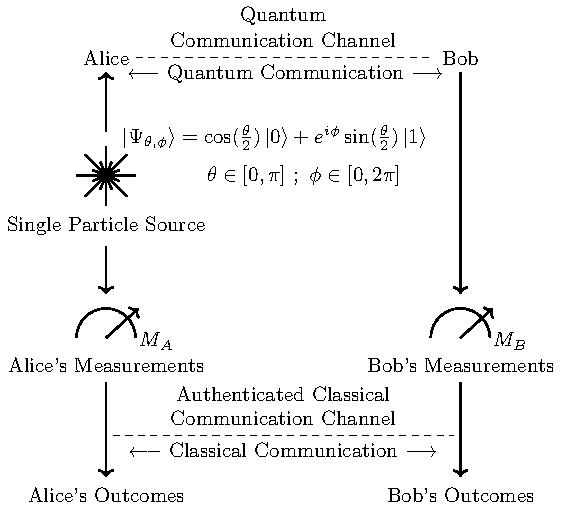
\includegraphics[width=0.95\linewidth, height=0.5\textheight]{figures/pdf/prepare-and-measure-qkd-protocol.pdf}
                    \vspace{-1.5ex}
                    \caption{\color{blue}{Figure 1a: }\color{black}{\tabular[t]{@{}l@{}}Schematic of a Prepare-and-Measure\\QKD protocol\endtabular}}
                    \label{fig:prepare-measure-qkd-protocol}
                \end{minipage}%
                \begin{minipage}{0.5\textwidth}
                    \centering
                    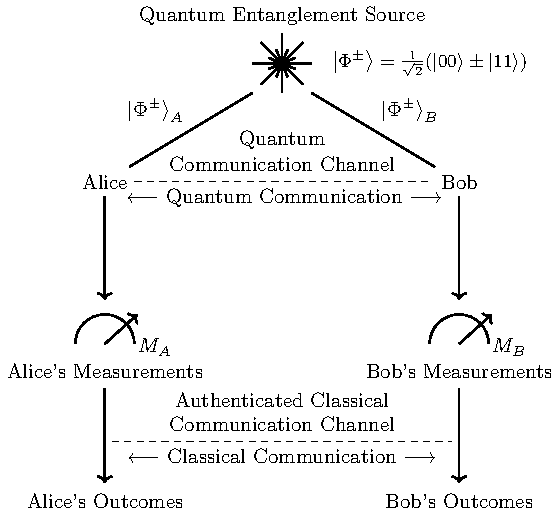
\includegraphics[width=0.95\linewidth, height=0.5\textheight]{figures/pdf/entanglement-based-qkd-protocol.pdf}
                    \vspace{-1.5ex}
                    \caption{\color{blue}{Figure 1b: }\color{black}{\tabular[t]{@{}l@{}}Schematic of an Entanglement-based\\QKD protocol\endtabular}}
                    \label{fig:entanglement-based-qkd-protocol}
                \end{minipage}
            \end{figure}
   
		\end{frame}

		\begin{frame}
			\frametitle{\large What is a Quantum Key Distribution (QKD) protocol?}

            \vspace{4ex}
            \begin{figure}
                \centering
                \begin{minipage}{0.4\textwidth}
                    \centering
                    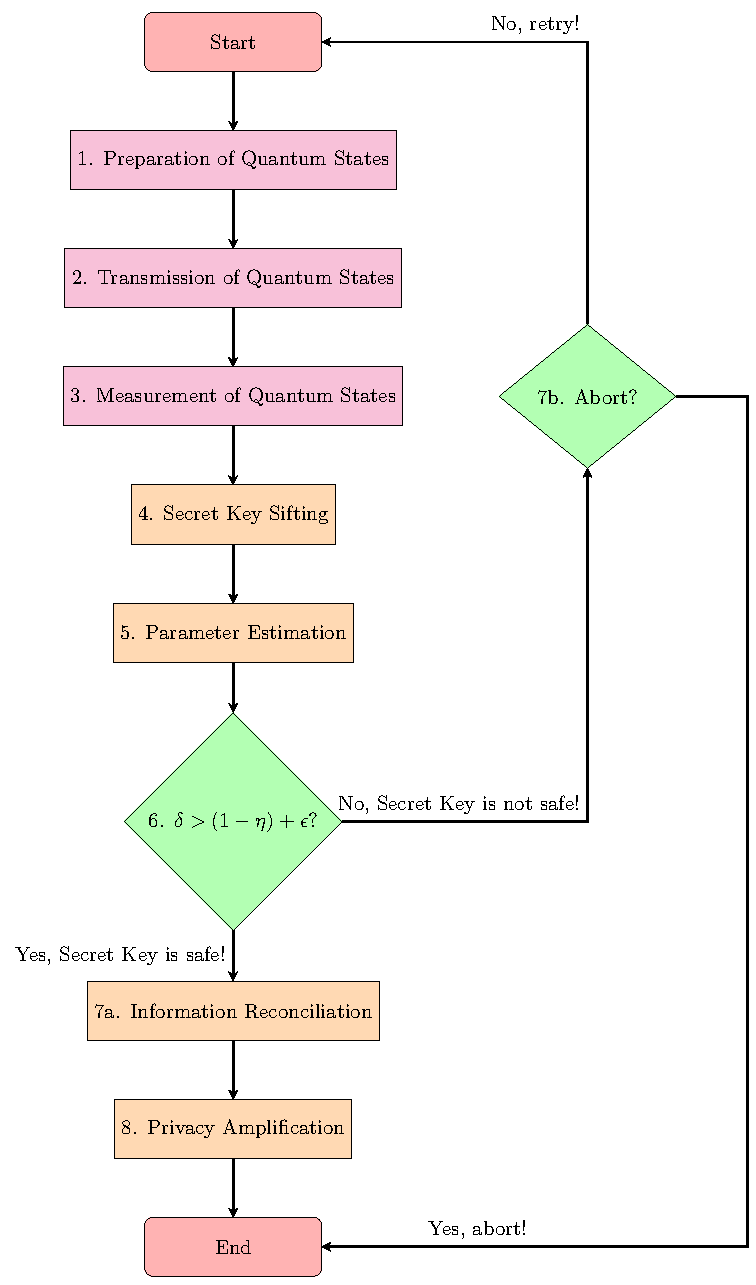
\includegraphics[width=1.0\linewidth, height=0.75\textheight]{figures/pdf/qkd-protocol-flowchart.pdf}
                    \vspace{-4ex}
                    \caption{\color{blue}{Figure 2: }\color{black}{Flowchart of a QKD protocol}}
                    \label{fig:qkd-protocol-flowchart-1}
                \end{minipage}%
                \hspace{0.05\textwidth}%
                \begin{minipage}{0.55\textwidth}
                    \begin{enumerate}\footnotesize
                        \item Preparation of Quantum States
                        \begin{itemize}\scriptsize
                            \item Single Particles, Entangled Particles, Coherent States, Fock States, etc.
                        \end{itemize}
                        \item Transmission of Quantum States
                        \begin{itemize}\scriptsize
                            \item Uses a quantum communication channel with a certain efficiency ${\eta}_{C}$
                            \item ``Flying'' quantum states can be eavesdropped, with noisy effects $\epsilon$
                        \end{itemize}
                        \item Measurement of Quantum States
                        \begin{itemize}\scriptsize
                            \item Uses quantum measurement devices with a certain efficiency ${\eta}_{D}$
                            \item Composes a raw key
                        \end{itemize}
                        \item Secret Key Sifting
                        \begin{itemize}\scriptsize
                            \item Identifies which protocol rounds can be used to compose a sifted key
                        \end{itemize}
                    \end{enumerate}
                \end{minipage}
            \end{figure}
   
		\end{frame}
  

		\begin{frame}
			\frametitle{\large What is a Quantum Key Distribution (QKD) protocol?}

            \vspace{4ex}
            \begin{figure}
                \centering
                \begin{minipage}{0.4\textwidth}
                    \centering
                    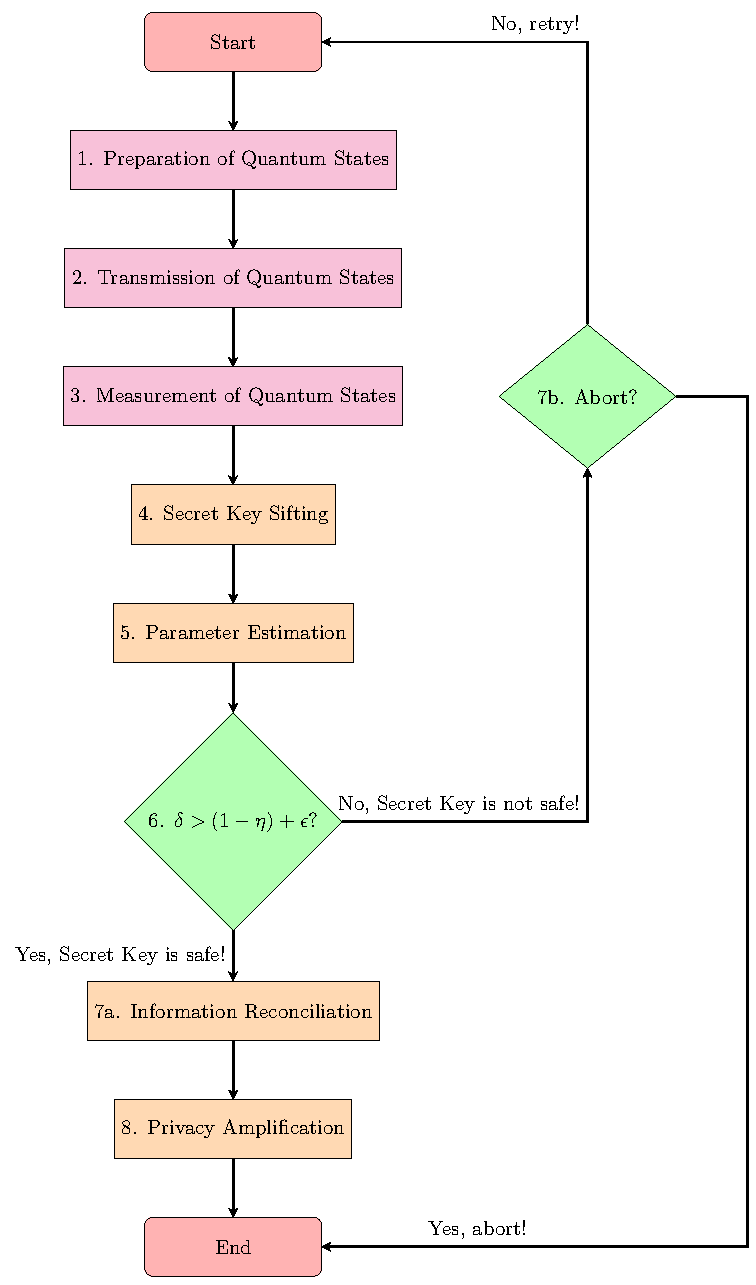
\includegraphics[width=1.0\linewidth, height=0.75\textheight]{figures/pdf/qkd-protocol-flowchart.pdf}
                    \vspace{-4ex}
                    \caption{\color{blue}{Figure 2: }\color{black}{Flowchart of a QKD protocol}}
                    \label{fig:qkd-protocol-flowchart-2}
                \end{minipage}%
                \hspace{0.05\textwidth}%
                \begin{minipage}{0.55\textwidth}
                    \begin{enumerate}\footnotesize
                        \item[5.] Parameter Estimation
                        \begin{itemize}\scriptsize
                            \item Samples and evaluates the Quantum Bit Error Rate (QBER) $\delta$ of the quantum communication channel
                            \item Estimates the key rate
                            \item Estimates the secure mutual information between Alice and Bob
                        \end{itemize}
                        \item[6.] (Eavesdropping detected?)\\$\Rightarrow$ $\delta > (1 - {\eta}_{C}) + (1 - {\eta}_{D}) + \epsilon$\ ?
                        \begin{enumerate}\scriptsize
                            \item[7a.] Yes! $\Rightarrow$ Information Reconciliation
                            \begin{itemize}\scriptsize
                                \item Applies an Error Correction Code (ECC) to correct the sifted into an error-free key
                                \item These ECC algorithms include:\\
                                - Cascade protocol, Winnow\\\hspace{1ex}protocol, and Low-Density\\\hspace{1ex}Parity-Check (LDPC) codes
                                \item Can be accelerated by classical software and hardware\\(e.g., OpenMP, CUDA, etc.)
                            \end{itemize}
                            \item[7b.] No! $\Rightarrow$ Abort? (or Retry?)
                        \end{enumerate}
                    \end{enumerate}
                \end{minipage}
            \end{figure}
   
		\end{frame}
  

		\begin{frame}
			\frametitle{\large What is a Quantum Key Distribution (QKD) protocol?}

            \vspace{4ex}
            \begin{figure}
                \centering
                \begin{minipage}{0.4\textwidth}
                    \centering
                    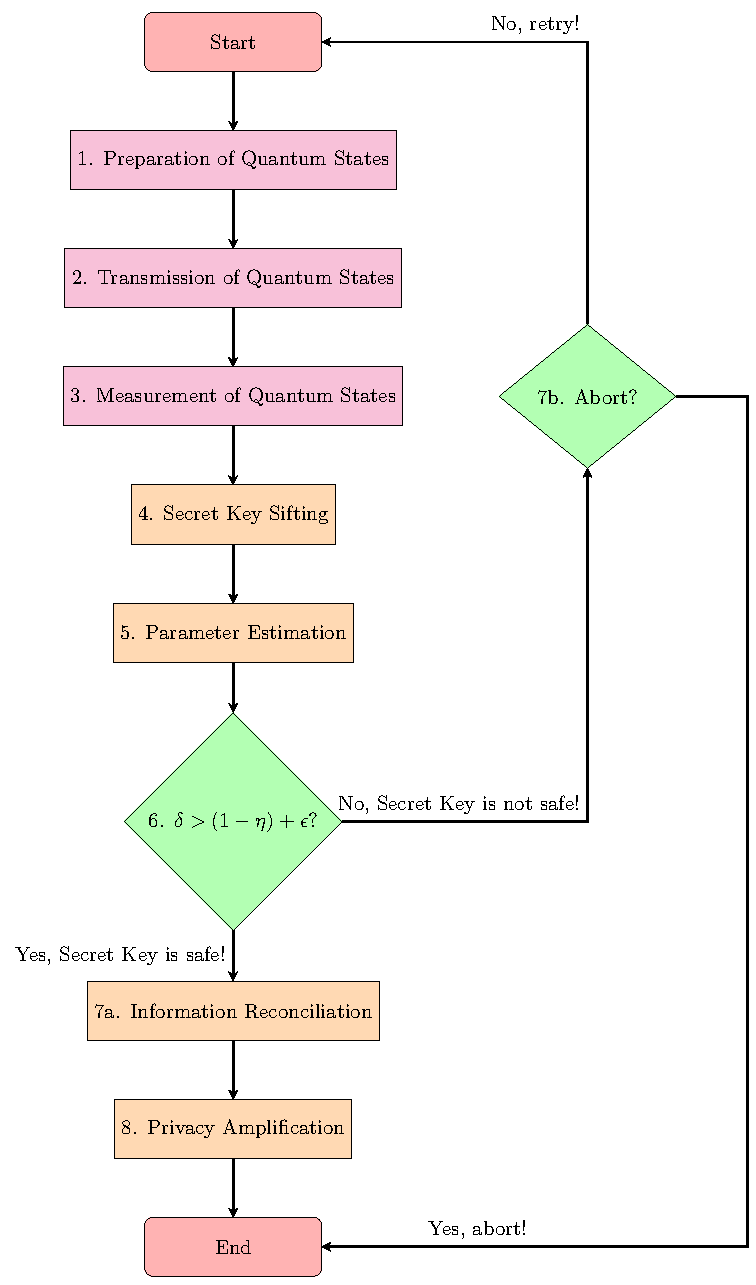
\includegraphics[width=1.0\linewidth, height=0.75\textheight]{figures/pdf/qkd-protocol-flowchart.pdf}
                    \vspace{-4ex}
                    \caption{\color{blue}{Figure 2: }\color{black}{Flowchart of a QKD protocol}}
                    \label{fig:qkd-protocol-flowchart}
                \end{minipage}%
                \hspace{0.05\textwidth}%
                \begin{minipage}{0.55\textwidth}
                    \begin{enumerate}\footnotesize
                        \item[8.] Privacy Amplification Estimation
                        \begin{itemize}\scriptsize
                            \item Applies a Universal Hash Function on the error-free key, composing the final (and amplified) secret key
                            \item This Universal Hash Function can be a Toeplitz Hashing procedure, usually applied using a random seed as well
                            \item Can be accelerated by classical software and hardware\\(e.g., OpenMP, CUDA, etc.)
                        \end{itemize}
                    \end{enumerate}

                    \begin{itemize}\footnotesize
                        \item The Secret Key Sifting, Parameter Estimation, Information Reconciliation, and Privacy Amplification steps require an authenticated and interactive exchange of classical information
                        \begin{itemize}\scriptsize
                            \item We can achieve it with\\ a Carter-Wegman Message Authentication Code (CW-MAC), requiring an initial small secret defined \textit{a priori}
                        \end{itemize}
                    \end{itemize}
                \end{minipage}
            \end{figure}
   
		\end{frame}

  
	\section{Problem}

		\begin{frame}
			\frametitle{\normalsize Can a QKD protocol with untrusted quantum devices be secure?}

            \begin{itemize}
                \item Considering Entanglement-based QKD protocols:
                \begin{itemize}\small
                    \item The entangled particles are emitted from a common source
                    \item The parties measure each particle on a randomly chosen basis
                    \item The measurement outcomes:
                    \begin{itemize}
                        \item Are kept private and secret
                        \item Compose the (initial) raw key
                    \end{itemize}
                    \item Here, we assume that:
                    \begin{itemize}
                        \item The locations of the parties (Alice and Bob) are secure
                        \item The parties (Alice and Bob) trust their measuring devices
                    \end{itemize}
                    \item The source of the entangled particles:
                    \begin{itemize}
                        \item It is not trusted by the parties (Alice and Bob)
                        \item Might be under the control of an eavesdropper (Eve)
                    \end{itemize}
                \end{itemize}
            \end{itemize}
		\end{frame}

		\begin{frame}
			\frametitle{\normalsize Can a QKD protocol with untrusted quantum devices be secure?}

            \vspace{2.5ex}
            \begin{itemize}
                \item Considering Entanglement-based QKD protocols:
                \begin{itemize}\small
                    \item The source of the entangled particles is \textbf{not trusted}:
                    \begin{itemize}
                        \item Example:\\
                         - The eavesdropper could replace the original\\\hspace{0.8ex} source of entangled particles by a new one\\
                         - This new source of entangled particles produces\\\hspace{0.8ex} quantum states that give it useful information \\\hspace{0.8ex} about the parties’ measurement outcomes
                        \item However, the parties (Alice and Bob) can...\\
                         1. Perform measurements in well-chosen\\\hspace{1.6ex} bases on a random subset of particles\\
                         2. Compare their measurement results\\
                         3. Estimate the quantum states\\\hspace{1.6ex} they receive from the eavesdropper\\
                         4. Decide whether a secret key can be\\\hspace{1.6ex} extracted from those quantum states
                    \end{itemize}
                \end{itemize}
            \end{itemize}
		\end{frame}

		\begin{frame}
			\frametitle{\normalsize Can a QKD protocol with untrusted quantum devices be secure?}

            \vspace{2.5ex}
            \begin{itemize}
                \item Considering Entanglement-based QKD protocols:
                \begin{itemize}\small
                    \item And about the cases that even the measuring devices\\ are \textbf{not trusted}?
                    \begin{itemize}
                        \item Examples:\\
                         - The measurement directions may drift\\\hspace{0.8ex} with time due to manufacture imperfections\\
                         - A malicious party might have fabricated them
                        \item In those cases, the parties (Alice and Bob)...\\
                         - Have no guarantee that the actual measurement\\\hspace{0.8ex}  bases correspond to the expected ones\\
                         - Cannot even make assumptions about\\\hspace{0.8ex}  the dimension of the Hilbert Space defined\\\hspace{0.8ex} in those physical apparatuses
                    \end{itemize}
                \end{itemize}
                \item QKD protocols can often ensure unconditional security
                \begin{itemize}
                    \item If combined with One-Time Pad (OTP)
                    \item But... They can be susceptible to side-channel attacks!
                \end{itemize}
            \end{itemize}
		\end{frame}

    \section{Motivation}

		\begin{frame}
			\frametitle{\footnotesize What is a Device‑Independent ‑ Quantum Key Distribution (DI‑QKD) protocol?}

            \vspace{2.5ex}
            \begin{itemize}
                \item Device‑Independent ‑ Quantum Key Distribution (DI‑QKD) is a concept of security for QKD protocols that:
                \begin{itemize}
                    \item Seeks to ensure the security of QKD protocols:
                    \begin{itemize}
                        \item Without considering any details about the internal working of the quantum devices being used\\
                        - Therefore, guarantees the security of a QKD protocol\\\hspace{0.5em}even when the quantum devices are imperfect,\\\hspace{0.5em}untrusted, or manipulated by a malicious party
                        \item Based on the violation of Bell Inequalities, ensuring that:\\
                        - There are quantum correlations between\\\hspace{0.5em}the quantum devices being used\\
                        - The security is inferred directly from those\\\hspace{0.5em}quantum correlations observed on the outcomes\\\hspace{0.5em}from the quantum measurement devices\\
                        - Do not exist any local hidden variables
                    \end{itemize}
                    \item It is considered a ``holy-grail'' on Quantum Cryptography!
                \end{itemize}
            \end{itemize}
		\end{frame}

		\begin{frame}
			\frametitle{\footnotesize What is a Device‑Independent ‑ Quantum Key Distribution (DI‑QKD) protocol?}

            \vspace{2.5ex}
            \begin{itemize}
                \item Device‑Independent ‑ Quantum Key Distribution (DI‑QKD) is a concept of security for QKD protocols that:
                \begin{itemize}
                    \item However... Needs basic assumptions to be ensured:
                    \begin{itemize}
                        \item The physical locations of the parties are secure\\
                        - No unwanted information can leak out to the outside
                        \item The parties have a Trusted Random Number Generator (TRNG), producing a classical random output\\
                        - Possibly, one derived from thermal noise or \\\hspace{0.5em}based on a Quantum Random Number Generator (QRNG)
                        \item The parties have trusted classical devices\\
                        - Capable of storing and processing the classical data\\\hspace{0.5em}generated by their quantum devices
                        \item The parties share a public authenticated\\classical communication channel\\
                        - The parties can start with a small shared secret
                        \item Quantum Mechanics is correct (and well-defined)
                    \end{itemize}
                \end{itemize}
            \end{itemize}
		\end{frame}

		\begin{frame}
			\frametitle{\footnotesize What is a Device‑Independent ‑ Quantum Key Distribution (DI‑QKD) protocol?}

            \vspace{2.5ex}
            \begin{itemize}
                \item How can DI-QKD protocols possibly be secure?
                \begin{itemize}
                    \item Some reasons lead the (usual) QKD protocols to\\ be insecure in Device-Independent scenarios:
                    \begin{itemize}
                        \item Sometimes they produce classical correlations\\
                        - We can reproduce them without\\\hspace{0.5em}invoking quantum mechanics at all\\
                        - We can generate them from a set of classical\\\hspace{0.5em}random data shared by the parties' systems
                        \vspace{1.5ex}
                        \item Those classical correlations can be written as:\\
                        - $P(ab|XY) = \sum_{\lambda} P(\lambda) \times D(a|X,\lambda) \times D(b|Y,\lambda)$\\
                        \vspace{0.75ex}\scriptsize
                        \hspace{0.6em}Where:\\
                        \hspace{0.75em}$\sbullet$ $\lambda$ is a classical variable with probability distribution\\
                        \hspace{1.15em}$P(\lambda)$, shared by the parties' quantum devices\\
                        \hspace{0.75em}$\sbullet$ $D(a|X,\lambda)$ is a function that completely specifies Alice's\\
                        \hspace{1.15em}outputs once the input $X$ and the variable $\lambda$ are given\\
                        \hspace{0.75em}$\sbullet$ $D(b|Y,\lambda)$ is a function that completely specifies Bob's\\
                        \hspace{1.15em}outputs once the input $Y$ and the variable $\lambda$ are given
                    \end{itemize}
                \end{itemize}
            \end{itemize}
		\end{frame}

		\begin{frame}
			\frametitle{\footnotesize What is a Device‑Independent ‑ Quantum Key Distribution (DI‑QKD) protocol?}

            \vspace{1ex}
            \begin{itemize}
                \item How can DI-QKD protocols possibly be secure?
                \begin{itemize}
                    \item Some reasons lead the (usual) QKD protocols to\\ be insecure in Device-Independent scenarios:
                    \begin{itemize}
                        \item A copy of the variable $\lambda$ will give the full information\\about the parties' outputs $a$ and $b$ to an eavesdropper\\ (Eve), once the inputs $X$ and $Y$ are announced
                        \vspace{1.5ex}
                        \item However... The strategy for these correlations is\\ not available to the eavesdropper if the outputs\\ $a$ and $b$ of the parties' quantum devices\\
                        - Are correlated in a non-local way\\
                        - Violate a Bell Inequality
                        \vspace{1ex}
                        \item Therefore, the violation of a Bell Inequality is a key requirement for the security of DI-QKD protocols!
                    \end{itemize}
                \end{itemize}
            \end{itemize}
		\end{frame}

    \section{Results}

		\begin{frame}
			\frametitle{\large What are the ingredients of a DI‑QKD protocol?}

            \vspace{3ex}
            \begin{itemize}
                \item Let's consider the following QKD protocol:
                \begin{itemize}
                    \item The parties (Alice and Bob) share a quantum communication channel between them
                    \begin{itemize}
                        \item Consisting of common source of entangled particles\\
                        - Producing an entangled Werner quantum state\\\hspace{0.5em}${\rho}_{AB} = p|{\Phi}^{+}\rangle\langle{\Phi}^{+}| + (1 - p) \frac{\mathbb{I}}{4}$\\
                        \vspace{0.75ex}\hspace{0.5em}Where: $|{\Phi}^{+}\rangle = \frac{1}{\sqrt{2}}(|00\rangle + |11\rangle)$ and\\\hspace{3.75em}the term $\frac{\mathbb{I}}{4}$ represents white noise 
                    \end{itemize}
                    \vspace{1.5ex}
                    \item The parties choose a measurement to apply to their particles for each round, resulting on binary outcomes
                    \begin{itemize}
                        \item Alice has three measurements choices: $X \in \{ {A}_{0}, {A}_{1}, {A}_{2}$ \}\\
                        - Where: ${A}_{0} = {\sigma}_{z}$, ${A}_{1} = \frac{({\sigma}_{z} + {\sigma}_{x})}{\sqrt{2}}$, ${A}_{2} = \frac{({\sigma}_{z} - {\sigma}_{x})}{\sqrt{2}}$
                        \item Bob has two measurements choices: $Y \in \{ {B}_{0}, {B}_{1} \}$\\
                        - Where: ${B}_{1} = {\sigma}_{z}$, ${B}_{2} = {\sigma}_{x}$
                        \item The binary outcomes are denoted as $\{+1 ,-1\}$
                    \end{itemize}
                \end{itemize}
            \end{itemize}
		\end{frame}

		\begin{frame}
			\frametitle{\large What are the ingredients of a DI‑QKD protocol?}

            \vspace{2.5ex}
            \begin{itemize}
                \item Let's consider the following QKD protocol:
                \begin{itemize}
                    \item Recall that:
                    \vspace{2ex}
                    \begin{itemize}
                        \item ${\rho}_{AB} = \begin{bmatrix}
                            \frac{(1 + p)}{4} & 0 & 0 & \frac{p}{2}\\
                            0 & \frac{(1 - p)}{4} & 0 & 0\\
                            0 & 0 & \frac{(1 - p)}{4} & 0\\
                            \frac{p}{2} & 0 & 0 & \frac{(1 + p)}{4}
                        \end{bmatrix}$
                    \end{itemize}
                    \hspace*{-7.5ex}
                    \begin{minipage}{0.5\textwidth}
                        \begin{itemize}
                            \item ${A}_{0} = {B}_{1} = {\sigma}_{z} =
                            \begin{bmatrix}
                                1 &  0 \\
                                0 & -1
                            \end{bmatrix}$
                            \vspace{2ex}
                            \item ${B}_{2} = {\sigma}_{x} = \begin{bmatrix}
                                0 & 1 \\
                                1 & 0
                            \end{bmatrix}$
                        \end{itemize}
                    \end{minipage}%
                    \hspace*{-2.5ex}
                    \begin{minipage}{0.5\textwidth}
                        \vspace{1.25ex}
                        \begin{itemize}
                            \item ${A}_{1} = \frac{({\sigma}_{z} + {\sigma}_{x})}{\sqrt{2}} = \begin{bmatrix}
                                 \frac{1}{\sqrt{2}} &  \frac{1}{\sqrt{2}} \\
                                 \frac{1}{\sqrt{2}} & -\frac{1}{\sqrt{2}}
                            \end{bmatrix}$
                            \vspace{2ex}
                            \item ${A}_{2} = \frac{({\sigma}_{z} - {\sigma}_{x})}{\sqrt{2}} = \begin{bmatrix}
                                 \frac{1}{\sqrt{2}} &  \frac{1}{\sqrt{2}} \\
                                 \frac{1}{\sqrt{2}} & -\frac{1}{\sqrt{2}}
                            \end{bmatrix}$
                        \end{itemize}
                    \end{minipage}

                    
                    
                \end{itemize}
            \end{itemize}
		\end{frame}

		\begin{frame}
			\frametitle{\large What are the ingredients of a DI‑QKD protocol?}
   
            \begin{itemize}
                \item Let's consider the following QKD protocol:
                \begin{itemize}
                    \item The (initial) raw key is extracted from the resulting\\ outcomes of the pair of measurements $\{{A}_{0}, {B}_{1}\}$
                    \begin{itemize}
                        \item The Quantum Bit Error Rate (QBER) is defined as:\\
                        $\sbullet$ $Q = P(a \neq b | 01) = P(a \neq b | {A}_{0}, {B}_{1}) =$\\
                        \hspace{1.4em}$= P(a = 0, b = 1 | {A}_{0}, {B}_{1}) + P(a = 1, b = 0 | {A}_{0}, {B}_{1})$\\
                        \vspace{1ex}
                        - Estimates the amount of quantum correlations\\
                        \hspace{0.5em}between the parties, using the same measurement\\
                        - Quantifies the amount of classical communication\\\hspace{0.5em}required for the Error Correction protocol/code\\\hspace{0.5em}during the Information Reconciliation step 
                    \end{itemize}
                \end{itemize}
            \end{itemize}
		\end{frame}

		\begin{frame}
			\frametitle{\large What are the ingredients of a DI‑QKD protocol?}

            \vspace{3ex}
            \begin{itemize}
                \item Let's consider the following QKD protocol:
                \begin{itemize}
                    \item The measurements ${A}_{1}$, ${A}_{2}$, ${B}_{1}$, and ${B}_{2}$ are\\ used on a subset of the particles to estimate\\ the Clauser-Horne-Shimony-Holt (CHSH) polynomial:
                    \begin{itemize}
                        \item $S = \langle {a}_{1} {b}_{1} \rangle + \langle {a}_{1} {b}_{2} \rangle + \langle {a}_{2} {b}_{1} \rangle - \langle {a}_{2} {b}_{2} \rangle$\\
                        \vspace{1ex}
                        - Where the correlators are defined as\\
                        \hspace{0.5em}$\langle {a}_{i} {b}_{j} \rangle = P(a = b | i,j) - P(a \neq b|i,j)$
                        \vspace{0.5em}
                        \item The CHSH polynomial is used by the parties to:\\
                        - Bound the eavesdropper's potential partial\\\hspace{0.5em}information about the (weak) error-free key\\
                        - Define how much secret information available to\\\hspace{0.5em}a potential eavesdropper needs to be reduced\\\hspace{0.5em}during the Privacy Amplification step
                    \end{itemize}
                    \item The parameters $Q$ and $S$ are used to estimate the information available to a potential eavesdropper
                \end{itemize}
            \end{itemize}
		\end{frame}

		\begin{frame}
			\frametitle{\large What are the ingredients of a DI‑QKD protocol?}

            \vspace{3ex}
            \begin{itemize}
                \item Let's consider the following QKD protocol:
                \begin{itemize}
                    \item The CHSH polynomial's correlations satisfy:
                    \begin{itemize}
                        \item $Q = \frac{1}{2} - \frac{p}{2} \Leftrightarrow \frac{p}{2} = \frac{1}{2} - Q \Leftrightarrow p = 1 - 2Q$
                        \item $S = 2 \sqrt{2} p = 2 \sqrt{2} (1 - 2Q)$
                    \end{itemize}
                    \item In order to bound the potential eavesdropper's available information, the parties do not need to assume that:
                    \begin{itemize}
                        \item They perform the measurements ${A}_{0}$, ${A}_{1}$, ${A}_{2}$, ${B}_{1}$, and ${B}_{2}$
                        \item The quantum systems ${\rho}_{AB}$ are of dimension $2$
                    \end{itemize}
                    \item Regarding the CHSH polynomial, we have:
                    \begin{itemize}
                        \item Classically correlated data, for $p \leq \frac{1}{\sqrt{2}}$, and thus, $S \leq 2$\\
                        - In this case, secure DI-QKD protocol is not possible
                        \item Maximal quantum violation, for $p = 1$, and thus, $S = 2\sqrt{2}$\\
                        - In this case, the potential eavesdropper has\\\hspace{0.5em}has no available information about the secret key
                        \item Now, we can interpolate for the range $\frac{1}{\sqrt{2}} < p \leq 2\sqrt{2}$\\ to prove the security of the DI-QKD protocol
                    \end{itemize}
                \end{itemize}
            \end{itemize}
		\end{frame}

		\begin{frame}
			\frametitle{\large How to prove the security of a DI‑QKD protocol?}

            \vspace{3ex}
            \begin{itemize}
                \item Let's consider the following eavesdropping strategies:
                \begin{itemize}
                    \item For the most general attacks:
                    \begin{itemize}
                        \item The only data available to the parties to\\ bound the eavesdropper's knowledge is:\\
                        - The observed relation between the inputs and outputs
                        \item No assumptions on the type of quantum measurements and quantum physical systems used are made
                        \vspace{2ex}
                        \item Generally, we can model these attacks as a tripartite entangled quantum state ${|\Psi\rangle}_{ABE} \in {\mathcal{H}}_{A}^{\otimes n} \otimes {\mathcal{H}}_{B}^{\otimes n} \otimes {\mathcal{H}}_{E}$\\
                        \vspace{0.75ex}
                        - Where: $n$ is the number of bits of the raw key
                        \vspace{2ex}
                        \item The size $d$ of the Hilbert Space of the parties'\\ quantum physical systems is:\\
                        - Unknown to the parties\\
                        - Fixed (and known) to the eavesdropper
                    \end{itemize}
                \end{itemize}
            \end{itemize}
		\end{frame}

		\begin{frame}
			\frametitle{\large How to prove the security of a DI‑QKD protocol?}

            \vspace{3ex}
            \begin{itemize}
                \item Let's consider the following eavesdropping strategies:
                \begin{itemize}
                    \item Focusing on collective attacks:
                    \begin{itemize}
                        \item The eavesdropper applies the same attack to\\ each quantum physical system of the parties\\
                        - The respective quantum states are \textit{independent and\\\hspace{0.5em}identically distributed} (\textit{i.i.d.}), and thus, ${|\Psi\rangle}_{ABE} = {|\psi\rangle}_{ABE}^{\otimes n}$
                        \item The quantum measurement devices\\
                        - Have no memory register\\
                        - Behave \textit{independent and identically distributed}\\\hspace{0.5em}(\textit{i.i.d.}) in every round of the QKD protocol
                        \vspace{2ex}
                        \item The (asymptotic) secret key rate $r$ has a lower bound\\ given by the Devetak-Winter key rate ${r}_{DW}$ formula:\\
                        $\sbullet$\, $r \geq {r}_{DW} = \underbrace{\strut I({A}_{0}:{B}_{1})}_{\substack{\text{Mutual information}\\ \text{between Alice and Bob}}} - \underbrace{\chi({B}_{1}:E)}_{\substack{\text{Holevo quantity}\\ \text{between Eve and Bob}}} $
                     \end{itemize}
                \end{itemize}
            \end{itemize}
		\end{frame}

		\begin{frame}
			\frametitle{\large How to prove the security of a DI‑QKD protocol?}

            \vspace{3ex}
            \begin{itemize}
                \item Let's consider the following eavesdropping strategies:
                \begin{itemize}
                    \item Focusing on collective attacks:
                    \begin{itemize}
                        \item The mutual information between Alice and Bob is given as:\\
                        \vspace{0.5ex}
                        $\sbullet$\, $I({A}_{0}:{B}_{1})\, = \underbrace{H({A}_{0})}_{\substack{\text{Individual (binary)}\\ \text{Shannon entropy}\\ \text{for Alice}}} + \underbrace{H({B}_{1})}_{\substack{\text{Individual (binary)}\\ \text{Shannon entropy}\\ \text{for Bob}}} - \underbrace{H({A}_{0},{B}_{1})}_{\substack{\text{Joint (binary)}\\ \text{Shannon entropy}\\ \text{for Alice and Bob}}}$
                        \vspace{0.75ex}
                        \item Since we assume uniform marginals, we also have:\\
                        \vspace{0.5ex}
                        $\sbullet$\, $I({A}_{0}:{B}_{1})\, = 1\ - \begin{rcases}H(Q)\,\end{rcases}\substack{\text{\scriptsize Individual (binary)}\\ \text{Shannon entropy on QBER}}$
                        \vspace{1.5ex}
                        \item The Holevo quantity between Eve and Bob is given as:\\
                        \vspace{0.5ex}
                        $\sbullet$\, $\chi({B}_{1}:E) = S({\rho}_{E}) - \frac{1}{2} \sum_{{b}_{1} = \pm 1} S({\rho}_{E|{b}_{1}})$\\
                        \vspace{1ex}
                        \footnotesize Where:\\
                        - ${\rho}_{E}$ denotes the Eve's quantum state after (partially) tracing out\\\hspace{0.5em}Alice and Bob's particles, i.e., ${\rho}_{E} = {Tr}_{AB}\left({|\psi\rangle}_{ABE}{\langle\psi|}_{ABE}\right)$\\
                        - ${\rho}_{E|{b}_{1}}$ denotes the Eve's quantum state when Bob has obtained\\\hspace{0.5em}the outcome result ${b}_{1}$ for the measurement setting ${B}_{1} = {\sigma}_{z}$
                     \end{itemize}
                \end{itemize}
            \end{itemize}
		\end{frame}

		\begin{frame}
			\frametitle{\large How to prove the security of a DI‑QKD protocol?}

            \vspace{4ex}
            \begin{itemize}
                \item Let's consider the following eavesdropping strategies:
                \begin{itemize}
                    \item Security against collective attacks:
                    \begin{itemize}
                        \item The optimal collective attack occurs when:\\
                        - The tripartite entangled quantum state ${|\psi\rangle}_{ABE}$\\\hspace{0.5em}is the purification of the (original) bipartite\\\hspace{0.5em}entangled quantum state ${\rho}_{AB}$\\
                        - The Holevo quantity $\chi({B}_{1}:E)$ achieves its possible\\\hspace{0.5em}largest value (compatible with the parameters $Q$ and $S$)
                    \end{itemize}
                    \vspace{1ex}
                    \item When the parties symmetrize their uniform marginals:
                    \begin{blockarray}{@{}p{5cm}\Right{\}}{\, \footnotesize Theorem for DI-QKD}}
                        \vspace{-\baselineskip}
                        \begin{itemize}
                            \item $\chi({B}_{1}:E) \leq h\left( \frac{1 + \sqrt{{(\frac{S}{2})}^{2} - 1}}{2} \right)$
                        \end{itemize}
                        \vspace*{-\baselineskip}
                        \vspace*{0.5ex}
                    \end{blockarray}
                    \vspace{-1ex}
                    \item Considering the optimal collective attack:
                    \begin{itemize}
                        \item We have to consider $\chi({B}_{1}:E) = h\left( \frac{1 + \sqrt{{(\frac{S}{2})}^{2} - 1}}{2} \right)$
                        \item The key rate is given by $r \geq 1 - h(Q) - h\left( \frac{1 + \sqrt{{(\frac{S}{2})}^{2} - 1}}{2} \right)$
                    \end{itemize}
                \end{itemize}
            \end{itemize}
		\end{frame}

		\begin{frame}
			\frametitle{\large How to prove the security of a DI‑QKD protocol?}

            \vspace{2ex}
            \begin{itemize}
                \item Simplifying the calculations for the DI-QKD protocol...
                \begin{itemize}
                    \item Recall that for the CHSH polynomial, we have:
                    \begin{itemize}
                        \item $S = 2 \sqrt{2}(1 - 2Q)$
                    \end{itemize}
                    \vspace{1ex}
                    \item We can simplify the (maximum) Holevo bound $\chi({B}_{1}:E)$\\ and Devetak-Winter key rate ${r}_{DW}$ for the DI-QKD protocol:
                    \begin{itemize}
                        \item $\chi({B}_{1}:E) = h\left( \frac{1 + \sqrt{{(\frac{S}{2})}^{2} - 1}}{2} \right) = h\left( \frac{1 + \sqrt{{\left(\frac{ 2 \sqrt{2}(1 - 2Q) }{2}\right)}^{2} - 1}}{2} \right)$
                        \item $r \geq {r}_{DW} = 1 - h(Q) - h\left( \frac{1 + \sqrt{{(\frac{S}{2})}^{2} - 1}}{2} \right) = $\\
                        \vspace{0.5ex}
                        \hspace{6.8ex}$= 1 - h(Q) - h\left( \frac{1 + \sqrt{{\left(\frac{ 2 \sqrt{2}(1 - 2Q) }{2}\right)}^{2} - 1}}{2} \right)$
                    \end{itemize}
                \end{itemize}
            \end{itemize}
            
		\end{frame}

		\begin{frame}
			\frametitle{\large How to prove the security of a DI‑QKD protocol?}

            \vspace{4ex}
            \begin{itemize}
                \item Simplifying the calculations for the (usual) Entanglement-based QKD protocol...
                \begin{itemize}
                    \item Recall that for the CHSH polynomial, we have:
                    \begin{itemize}\footnotesize
                        \item $S = 2 \sqrt{2}(1 - 2Q)$
                    \end{itemize}
                    \vspace{0.5ex}
                    \item The respective Holevo bound is given as follows:
                    \begin{itemize}\footnotesize
                        \item $\chi({B}_{1}:E) \leq h\left( Q + \frac{S}{2 \sqrt{2}} \right)$
                    \end{itemize}
                    \vspace{0.5ex}
                    \item We can simplify the (maximum) Holevo bound $\chi({B}_{1}:E)$\\ and the Devetak-Winter key rate ${r}_{DW}$ for the (usual) Entanglement-based QKD protocol:
                    \begin{itemize}\footnotesize
                        \item $\chi({B}_{1}:E) = h\left( Q + \frac{S}{2 \sqrt{2}} \right) = h\left( Q + \frac{2 \sqrt{2}(1 - 2Q)}{2 \sqrt{2}} \right) = $\\
                        \vspace{0.5ex}
                        \hspace{8ex}
                        $ = h\left( Q + (1 - 2Q) \right) = h\left( 1 - Q \right)$
                        \item $r \geq {r}_{DW} = 1 - h(Q) - h\left( Q + \frac{S}{2 \sqrt{2}} \right) = $\\
                        \vspace{0.25ex}
                        \hspace{6.8ex}$= 1 - h(Q) - h\left( Q + \frac{2 \sqrt{2}(1 - 2Q)}{2 \sqrt{2}} \right)$\\
                        \vspace{0.25ex}
                        \hspace{6.8ex}$= 1 - h(Q) - h\left( Q + (1 - 2Q) \right) = 1 - h(Q) - h(1 - Q)$\\
                    \end{itemize}
                \end{itemize}
            \end{itemize}
            
		\end{frame}

		\begin{frame}
			\frametitle{\large How to prove the security of a DI‑QKD protocol?}

            \vspace{4ex}
            \begin{itemize}
                \item What are the differences between the (usual) Entanglement-based QKD and DI-QKD protocols?
            \end{itemize}
            
            \begin{minipage}{0.5\textwidth}
                \centering
                \vspace{0.5ex}
                \scriptsize
                $\sbullet$\, For Holevo bounds:\\
                \vspace{0.25ex}
                \tiny
                - Greater Holevo bounds for the DI-QKD protocol\\
                - We can easily detect the presence of an eavesdropper\\for the DI-QKD protocol, allowing to better tolerate a QBER,\\ in comparison to the Entanglement-Based QKD protocol\\
                - For a QBER $Q$ around $14\%$, the eavesdropper has all\\ the information about the raw key in the DI-QKD protocol
                \vspace{-1.2ex}
                \begin{figure}
                    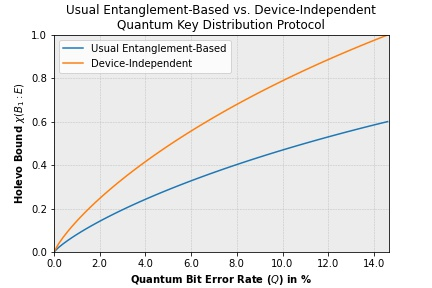
\includegraphics[width=\linewidth]{figures/jpg/holevo-bounds-plot.jpg}
                    \vspace{-4ex}
                \caption{\color{blue}{Figure 3: }\color{black}{Holevo bounds with respect to QBER $Q$}}
                \end{figure}
            \end{minipage}%
            \begin{minipage}{0.5\textwidth}
                \centering
                \vspace{0.5ex}
                \scriptsize $\sbullet$\, For Devetak-Winter key rates:\\
                \vspace{0.25ex}
                \tiny
                - Lower Devetak-Winter key rates for the DI-QKD protocol\\
                - The noise introduced by the eavesdropper will have greater impact on the DI-QKD protocol, reducing more the key rate,\\ compared to the Entanglement-Based QKD protocol\\
                - For a QBER $Q$ around $7\%$, no extractable secure raw key\\ will be possible in the DI-QKD protocol
                \vspace{-1.2ex}
                \begin{figure}
                    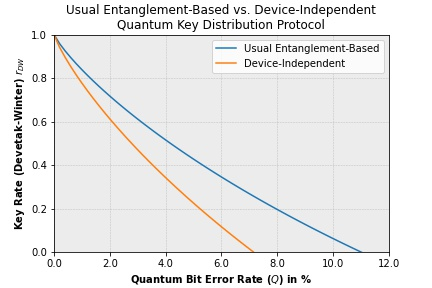
\includegraphics[width=\linewidth]{figures/jpg/key-rates-bounds-plot.jpg}
                    \vspace{-4ex}
                    \caption{\color{blue}{Figure 4: }\color{black}{Devetak-Winter key rates with respect to QBER $Q$}}
                \end{figure}
            \end{minipage}
            
		\end{frame}

    \section{Conclusion}

\end{document}